\documentclass[../main.tex]{subfiles}

\begin{document}
\chapter{Optimization}
\label{cha:cha_7}
\begin{center}
\Large{\textbf{CHAPTER OBJECTIVES}}
\end{center}

The primary objective of this chapter is to introduce you to how optimization can be
used to determine minima and maxima of both one-dimensional and multidimensional
functions. Specific objectives and topics covered are
\begin{itemize}
\item Understanding why and where optimization occurs in engineering and scientific
problem solving.
\item Recognizing the difference between one-dimensional and multidimensional
optimization.
\item Distinguishing between global and local optima.
\item Knowing how to recast a maximization problem so that it can be solved with a
minimizing algorithm.
\item Being able to define the golden ratio and understand why it makes onedimensional
optimization efficient.
\item Locating the optimum of a single-variable function with the golden-section search.
\item Locating the optimum of a single-variable function with parabolic interpolation.
\item Knowing how to apply the \texttt{fminbnd} function to determine the minimum of a
one-dimensional function.
\item Being able to develop MATLAB contour and surface plots to visualize twodimensional
functions.
\item Knowing how to apply the \texttt{fminsearch} function to determine the minimum of a
multidimensional function.

\end{itemize}

\newpage

\Large{YOU'VE GOT A PROBLEM}

\smallskip
\color{black}
\normalsize{An object like a bungee jumper can be projected upward at a specified velocity. If it
is subject to linear drag, its altitude as a function of time can be computed as}
\smallskip
\begin{center}
\large{$\ z=z_0+\dfrac{m}{c}(v_0+\dfrac{mg}{c})(1-e^{-(c/m)t})-\dfrac{mg}{c}t$} \hfill {(7.1)}
\normalsize
\end{center}
\begin{figure}[H]
	\centering
	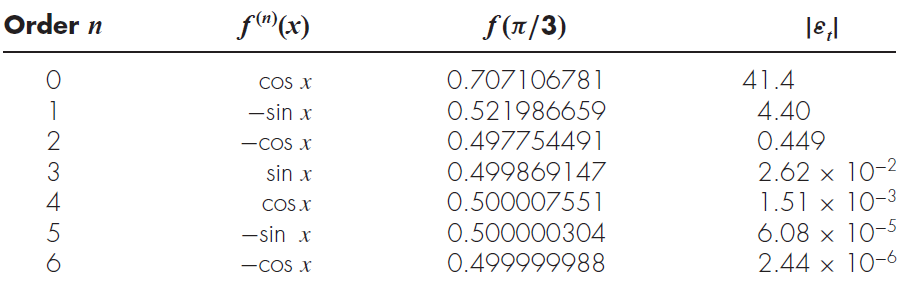
\includegraphics[width=0.6\linewidth]{fig_7_1}
	\caption{\textsf{Elevation as a function of time for an object initially projected upward with an initial velocity.}}
	\label{fig:fig_7_1}
\end{figure}
where $z$ = altitude (m) above the earth's surface (defined as $z$ = 0), $z_0$ = the initial altitude
(m), $m$ = mass (kg), $c$ = a linear drag coefficient (kg/s), $v_0$ = initial velocity (m/s), and $t$ =
time (s). Note that for this formulation, positive velocity is considered to be in the upward
direction. Given the following parameter values: $g = 9.81 m/s^2$, $z_0$ = 100 m, $v_0$ = 55 m/s,
$m$ = 80 kg, and $c$ = 15 kg/s, Eq. (7.1) can be used to calculate the jumper's altitude. As
displayed in Fig. 7.1, the jumper rises to a peak elevation of about 190 m at about $t$ = 4 s.
Suppose that you are given the job of determining the exact time of the peak elevation.
The determination of such extreme values is referred to as optimization. This chapter will
introduce you to how the computer is used to make such determinations.\bigskip

\section{INTRODUCTION AND BACKGROUND}
\label{sec:sec_7_1}

In the most general sense, optimization is the process of creating something that is as
effective as possible. As engineers, we must continuously design devices and products that
perform tasks in an efficient fashion for the least cost. Thus, engineers are always confronting
optimization problems that attempt to balance performance and limitations. In
addition, scientists have interest in optimal phenomena ranging from the peak elevation of
projectiles to the minimum free energy.

From a mathematical perspective, optimization deals with finding the maxima and
minima of a function that depends on one or more variables. The goal is to determine the
values of the variables that yield maxima or minima for the function. These can then be
substituted back into the function to compute its optimal values.

Although these solutions can sometimes be obtained analytically, most practical
optimization problems require numerical, computer solutions. From a numerical standpoint,
optimization is similar in spirit to the root-location methods we just covered in
Chaps. 5 and 6. That is, both involve guessing and searching for a point on a function. The
fundamental difference between the two types of problems is illustrated in Fig. 7.2. Root
location involves searching for the location where the function equals zero. In contrast,
optimization involves searching for the function's extreme points.

\begin{figure}[H]
	\centering
	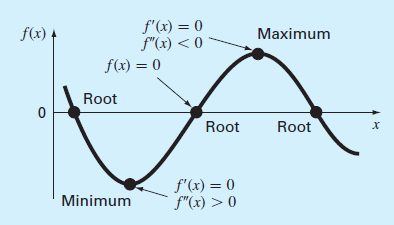
\includegraphics[width=0.5\linewidth]{fig_7_2}
	\caption{\textsf{A function of a single variable illustrating the difference between roots and optima.}}
	\label{fig:fig_7_2}
\end{figure}

As can be seen in Fig. 7.2, the optimums are the points where the curve is flat. In mathematical
terms, this corresponds to the x value where the derivative $f'(x)$ is equal to zero. Additionally, the second derivative,
$f''(x)$, indicates whether the optimum is a minimum or a maximum: if $f''(x) > 0$, 
the point is a maximum; if $f''(x) > 0$, the point is a minimum.

Now, understanding the relationship between roots and optima would suggest a possible
strategy for finding the latter. That is, you can differentiate the function and locate the
root (i.e., the zero) of the new function. In fact, some optimization methods do just this by
solving the root problem: $f''(x)$ = 0.
\newline

\begin{example}
	\textbf{Determining the Optimum Analytically by Root Location}
	\smallskip
	
	\noindent Problem Statement:
	Determine the time and magnitude of the peak elevation based on
	Eq. (7.1). Use the following parameter values for your calculation: $g = 9.81 m/s^2$,
	z0 = 100 m, v0 = 55 m/s, m = 80 kg, and c = 15 kg/s.

	\noindent Solution: Equation (7.1) can be differentiated to give.
	\medskip

	$\dfrac{dz}{dt}=v_0e^{-(c/m)t}-\dfrac{mg}{c}(1-e^{-(c/m)t})$ \hfill{E7.1.1}
	\medskip

	\noindent Note that because $v = dz/dt$, this is actually the equation for the velocity. The maximum
	elevation occurs at the value of t that drives this equation to zero. Thus, the problem
	amounts to determining the root. For this case, this can be accomplished by setting the derivative
	to zero and solving Eq. (E7.1.1) analytically for
	\medskip

	$t = \dfrac{m}{c}ln(1+\dfrac{cv_0}{mg})$
	\medskip

	\noindent Substituting the parameters gives
	\medskip

	$t=\dfrac{80}{15}ln(1+\dfrac{15(55)}{80(9.81)})=3.83166s$
	\medskip

	\noindent This value along with the parameters can then be substituted into Eq. (7.1) to compute the
	maximum elevation as
	\medskip

	\noindent $z=100+\dfrac{80}{15}(50+\dfrac{80(9.81)}{15})(1-e^{-(15/80)3.83166})-\dfrac{80(9.81)}{15}(3.83166)=192.8609m$                      
	\medskip

	We can verify that the result is a maximum by differentiating Eq. (E7.1.1) to obtain the
	second derivative
	\medskip

	$\dfrac{d^2z}{dt^2}=-\dfrac{c}{m}v_0e^{-(c/m)t}-ge^{-(c/m)t}=-9.81\dfrac{m}{s^2} $
	\medskip

	\noindent The fact that the second derivative is negative tells us that we have a maximum. Further,
	the result makes physical sense since the acceleration should be solely equal to the force of
	gravity at the maximum when the vertical velocity (and hence drag) is zero.

	Although an analytical solution was possible for this case, we could have obtained the
	same result using the root-location methods described in Chaps. 5 and 6. This will be left
	as a homework exercise.
	\newline
\end{example}

\color{black}

Although it is certainly possible to approach optimization as a roots problem, a variety
of direct numerical optimization methods are available. These methods are available for both
one-dimensional and multidimensional problems. As the name implies, one-dimensional
problems involve functions that depend on a single dependent variable. As in Fig. 7.3a, the
search then consists of climbing or descending one-dimensional peaks and valleys. Multidimensional
problems involve functions that depend on two or more dependent variables.

\begin{figure}[H]
	\centering
	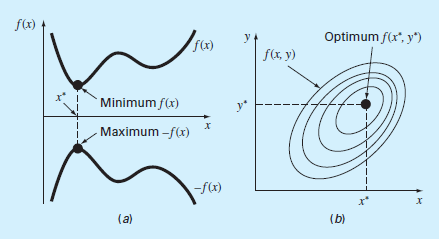
\includegraphics[width=0.5\linewidth]{fig_7_3}
	\caption{\textsf{(a) One-dimensional optimization. This figure also illustrates how minimization of $f(x)$ is
	equivalent to the maximization of $-f(x)$. (b) Two-dimensional optimization. Note that this
	figure can be taken to represent either a maximization (contours increase in elevation up to
	the maximum like a mountain) or a minimization (contours decrease in elevation down to the
	minimum like a valley).}}
	\label{fig:fig_7_3}
\end{figure}

In the same spirit, a two-dimensional optimization can again be visualized as searching out
peaks and valleys (Fig. 7.3b). However, just as in real hiking, we are not constrained to walk
a single direction; instead the topography is examined to efficiently reach the goal.

Finally, the process of finding a maximum versus finding a minimum is essentially
identical because the same value $x*$ both minimizes $f(x)$ and maximizes $-f(x)$. This
equivalence is illustrated graphically for a one-dimensional function in Fig. 7.3a.

In the next section, we will describe some of the more common approaches for onedimensional
optimization. Then we will provide a brief description of how MATLAB can
be employed to determine optima for multidimensional functions.\bigskip


\section{ONE-DIMENSIONAL OPTIMIZATION}
\label{sec:sec_7_2}

This section will describe techniques to find the minimum or maximum of a function of a
single variable $f(x)$. A useful image in this regard is the one-dimensional ''roller
coaster'' -like function depicted in Fig. 7.4. Recall from Chaps. 5 and 6 that root location
was complicated by the fact that several roots can occur for a single function. Similarly,
both local and global optima can occur in optimization.

A \textit{global optimum} represents the very best solution. A \textit{local optimum}, though not the
very best, is better than its immediate neighbors. Cases that include local optima are called
\textit{multimodal}. In such cases, we will almost always be interested in finding the global optimum.
In addition, we must be concerned about mistaking a local result for the global optimum.

Just as in root location, optimization in one dimension can be divided into bracketing
and open methods. As described in the next section, the golden-section search is an example
of a bracketing method that is very similar in spirit to the bisection method for root location.
This is followed by a somewhat more sophisticated bracketing approach-parabolic interpolation.
We will then show how these two methods are combined and implemented with
MATLAB's \texttt{fminbnd} function.

\begin{figure}[H]
	\centering
	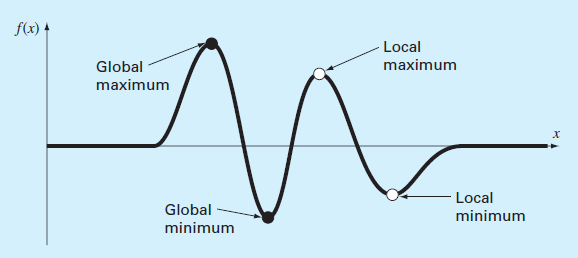
\includegraphics[width=0.75\linewidth]{fig_7_4}
	\caption{\textsf{(a) A function that asymptotically approaches zero at plus and minus $\infty$ and has two maximum and
	two minimum points in the vicinity of the origin. The two points to the right are local optima,
	whereas the two to the left are global.}}
	\label{fig:fig_7_4}
\end{figure}

\subsection{Golden-Section Search}

In many cultures, certain numbers are ascribed magical qualities. For example, we in theWest
are all familiar with ``lucky 7'' and ``Friday the 13th.'' Beyond such superstitious quantities,
there are several well-known numbers that have such interesting and powerful mathematical
properties that they could truly be called ``magical''. The most common of these are the ratio
of a circle's circumference to its diameter $\pi$ and the base of the natural logarithm $e$.

Although not as widely known, the golden ratio should surely be included in the pantheon
of remarkable numbers. This quantity, which is typically represented by the Greek
letter $\phi$ (pronounced: fee), was originally defined by Euclid (ca. 300 BCE) because of its
role in the construction of the pentagram or five-pointed star. As depicted in Fig. 7.5,
Euclid's definition reads: ``A straight line is said to have been cut in extreme and mean ratio
when, as the whole line is to the greater segment, so is the greater to the lesser.''

The actual value of the golden ratio can be derived by expressing Euclid's definition as
\medskip

$\dfrac{l_1+l_2}{l_1}=\dfrac{l_1}{l_2}$ \hfill {(7.2)}
\medskip

\noindent Multiplying by $l_1/l_2$ and collecting terms yields
\medskip

$\phi^2-\phi-1=0$ \hfill {(7.3)}
\medskip

\noindent where $\phi=l_1/l_2$. The positive root of this equation is the golden ratio:

$\phi = \dfrac{1+\sqrt{5}}{2}=1.61803398874989...$ \hfill {(7.4)}
\medskip

The golden ratio has long been considered aesthetically pleasing in Western cultures.
In addition, it arises in a variety of other contexts including biology. For our purposes, it
provides the basis for the golden-section search, a simple, general-purpose method for determining
the optimum of a single-variable function.

The golden-section search is similar in spirit to the bisection approach for locating
roots in Chap. 5. Recall that bisection hinged on defining an interval, specified by a lower
guess $(x_l)$ and an upper guess $(x_u)$ that bracketed a single root. The presence of a root between
these bounds was verified by determining that $f(x_l)$ and $f(x_u)$ had different signs.
The root was then estimated as the midpoint of this interval:
\medskip

$x_r=\dfrac{x_l+x_u}{2}$ \hfill {(7.5)}
\medskip

\begin{figure}[H]
	\centering
	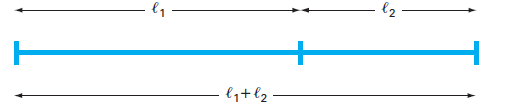
\includegraphics[width=0.65\linewidth]{fig_7_5}
	\caption{\textsf{Euclid's definition of the golden ratio is based on dividing a line into two segments so that the
	ratio of the whole line to the larger segment is equal to the ratio of the larger segment to the
	smaller segment. This ratio is called the golden ratio.}}
	\label{fig:fig_7_5}
\end{figure}

The final step in a bisection iteration involved determining a new smaller bracket. This was
done by replacing whichever of the bounds $x"_l$ or $x_u$ had a function value with the same sign
as $f(x_r)$. Akey advantage of this approach was that the new value $x_r$ replaced one of the old
bounds.

Now suppose that instead of a root, we were interested in determining the minimum of
a one-dimensional function. As with bisection, we can start by defining an interval that
contains a single answer. That is, the interval should contain a single minimum, and hence
is called \textit{unimodal}. We can adopt the same nomenclature as for bisection, where $x_l$ and $x_u$
defined the lower and upper bounds, respectively, of such an interval. However, in contrast
to bisection, we need a new strategy for finding a minimum within the interval. Rather than
using a single intermediate value (which is sufficient to detect a sign change, and hence a
zero), we would need two intermediate function values to detect whether a minimum
occurred.

The key to making this approach efficient is the wise choice of the intermediate points.
As in bisection, the goal is to minimize function evaluations by replacing old values with
new values. For bisection, this was accomplished by choosing the midpoint. For the
golden-section search, the two intermediate points are chosen according to the golden
ratio:
\smallskip

$x_1=x_l+d$ \hfill {(7.6)}

\smallskip
$x_2=x_u-d$ \hfill {(7.7)}

\noindent where
\smallskip

$d=(\phi-1)(x_u-x_l)$ \hfill {(7.8)}
\smallskip

\noindent The function is evaluated at these two interior points. Two results can occur:
\begin{enumerate}
	\item If, as in Fig. 7.6a, $f(x_1)<f(x_2)$, then $f(x_1)$ is the minimum, and the domain of $x$ to the
	left of $x_2$, from $x_l$ to $x_2$, can be eliminated because it does not contain the minimum. For
	this case, $x_2$ becomes the new $x_l$ for the next round.
	\item If $f(x_2)<f(x_1)$, then $f(x_2)$ is the minimum and the domain of $x$ to the right of $x_1$, from
	$x_1$ to $x_u$ would be eliminated. For this case, $x_1$ becomes the new $x_u$ for the next round.
\end{enumerate}

Now, here is the real benefit from the use of the golden ratio. Because the original $x_1$
and $x_2$ were chosen using the golden ratio, we do not have to recalculate all the function
values for the next iteration. For example, for the case illustrated in Fig. 7.6, the old $x_1$ becomes
the new $x_2$. This means that we already have the value for the new $f(x_2)$, since it is
the same as the function value at the old $x_1$.

To complete the algorithm, we need only determine the new $x_1$. This is done with
Eq. (7.6) with $d$ computed with Eq. (7.8) based on the new values of $x_l$ and $x_u$. A similar
approach would be used for the alternate case where the optimum fell in the left subinterval.
For this case, the new $x_2$ would be computed with Eq. (7.7).

As the iterations are repeated, the interval containing the extremum is reduced rapidly.
In fact, each round the interval is reduced by a factor of $\phi$ - 1(about 61.8\%). That means
that after 10 rounds, the interval is shrunk to about $0.618^{10}$ or 0.008 or 0.8\% of its initial
length. After 20 rounds, it is about 0.0066\%. This is not quite as good as the reduction
achieved with bisection (50\%), but this is a harder problem.

\begin{figure}[H]
	\centering
	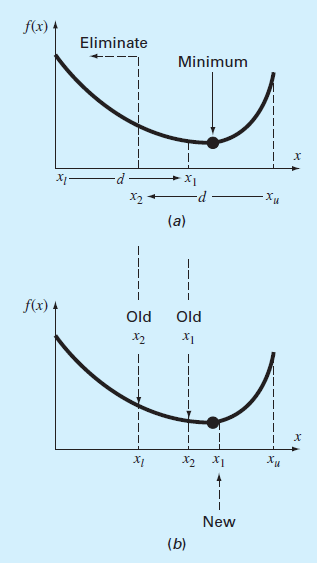
\includegraphics[width=0.4\linewidth]{fig_7_6}
	\caption{\textsf{(a) The initial step of the golden-section search algorithm involves choosing two interior points
	according to the golden ratio. (b) The second step involves defining a new interval that
	encompasses the optimum.}}
	\label{fig:fig_7_6}
\end{figure}


\begin{example}
	\textbf{Golden-Section Search}
	\smallskip
	
	\noindent Problem Statement:
	Use the golden-section search to find the minimum of

	$f(x)=\dfrac{x^2}{10}-2sin{x}$

	\noindent within the interval from $x_l=0$ to $x_u=4$

	\noindent Solution: First, the golden ratio is used to create the two interior points:
	\medskip

	$d = 0.61803(4 - 0) = 2.4721$
	\medskip

	$x_1 = 0 + 2.4721 = 2.4721$
	\medskip

	$x_2 = 4 - 2.4721 = 1.5279$
	\medskip

	\noindent The function can be evaluated at the interior points:
	\medskip

	$f(x_2) = \dfrac{1.5279^2}{10}-2sin(1.5279) = -1.7647)$
	\medskip

	$f(x_1) = \dfrac{2.4721^2}{10}-2sin(2.4721) = -0.6300)$
	\medskip

	Because $f(x_2)< f(x_1)$, our best estimate of the minimum at this point is that it is
	located at $x$ = 1.5279 with a value of $f(x) = -1.7647$. In addition, we also know that the
	minimum is in the interval defined by $x_l$, $x_2$, and $x_1$. Thus, for the next iteration, the lower
	bound remains $x_l = 0$, and $x_1$ becomes the upper bound, that is, $x_u = 2.4721$. In addition,
	the former $x_2$ value becomes the new $x_1$, that is, $x_1 = 1.5279$. In addition, we do not have to
	recalculate $f(x_1)$, it was determined on the previous iteration as $f(1.5279)=-1.7647$.

	All that remains is to use Eqs. (7.8) and (7.7) to compute the new value of $d$ and $x_2$:
	\medskip

	$d = 0.61803(2.4721 - 0) = 1.5279$
	\medskip

	$x_2 = 2.4721 - 1.5279 = 0.9443$

	\newpage
	The function evaluation at $x_2$ is $f(0.9943) = -1.5310$. Since this value is less than the
	function value at x1, the minimum is $f(1.5279) = -1.7647$, and it is in the interval prescribed
	by $x_2$, $x_1$, and $x_u$. The process can be repeated, with the results tabulated here:
	
	$$
	\begin{tabular}{|c|c|c|c|c|c|c|c|c|c|}
		\hline $i$ & $x_l$ & $f(x_l)$ & $x_2$ & $f(x_2)$ & $x_l$ & $f(x_l)$ & $x_u$ & $f(x_u)$ & $d$ \\
		\hline 1 & 0 & 0 & 1.5279 & -1.7647 & 2.4721 & -0.6300 & 4.0000 & 3.1136 & 2.4721 \\
		\hline 2 & 0 & 0 & 0.9443 & -1.5310 & 1.5279 & -1.7647 & 2.4721 & -0.6300 & 1.5279 \\
		\hline 3 & 0.9443 & -1.5310 & 1.5279 & -1.7647 & 1.8885 & -1.5432 & 2.4721 & -0.6300 & 0.9443 \\
		\hline 4 & 0.9443 & -1.5310 & 1.3050 & -1.7595 & 1.5279 & -1.7647 & 1.8885 & -1.5432 & 0.5836 \\
		\hline 5 & 1.3050 & -1.7595 & 1.5279 & -1.7647 & 1.6656 & -1.7136 & 1.8885 & -1.5432 & 0.3607 \\
		\hline 6 & 1.3050 & -1.7595 & 1.4427 & -1.7755 & 1.5279 & -1.7647 & 1.6656 & -1.7136 & 0.2229 \\
		\hline 7 & 1.3050 & -1.7595 & 1.3901 & -1.7742 & 1.4427 & -1.7755 & 1.5279 & -1.7647 & 0.1378 \\
		\hline 8 & 1.3901 & -1.7742 & 1.4427 & -1.7755 & 1.4752 & -1.7732 & 1.5279 & -1.7647 & 0.0851 \\
		\hline
	\end{tabular}
	$$
	
	\color{black} Note that the current minimum is highlighted for every iteration. After the eighth
	iteration, the minimum occurs at $x$ = 1.4427 with a function value of -1.7755. Thus, the
	result is converging on the true value of -1.7757 at $x$ = 1.4276.
	\newline
\end{example}

Recall that for bisection (Sec. 5.4), an exact upper bound for the error can be calculated
at each iteration. Using similar reasoning, an upper bound for golden-section search
can be derived as follows: Once an iteration is complete, the optimum will either fall in one
of two intervals. If the optimum function value is at $x_2$, it will be in the lower interval ($x_l,
x_2, x_1$). If the optimum function value is at $x_1$, it will be in the upper interval ($x_2, x_1, x_u$).
Because the interior points are symmetrical, either case can be used to define the error.

Looking at the upper interval ($x_2, x_1, x_u$), if the true value were at the far left, the maximum
distance from the estimate would be

$\Delta x_a = x_1 - x_2$
\medskip

$=x_l + (\phi - 1)(x_u - x_l ) - x_u + (\phi - 1)(x_u - x_l )$
\medskip

$=(x_l - x_u) + 2(\phi - 1)(x_u - x_l )$
\medskip

$=(2\phi - 3)(x_u - x_l )$
\medskip

\noindent or 0.2361 ($x_u - x_l$). If the true value were at the far right, the maximum distance from the
estimate would be

$\Delta x_b = x_u - x_1$
\medskip

$=x_u - x_l - (\phi - 1)(x_u - x_l )$
\medskip

$=(x_u - x_l) - (\phi - 1)(x_u - x_l )$
\medskip

$=(2 -\phi)(x_u - x_l)$
\medskip

\noindent or 0.3820 ($x_u - x_l$). Therefore, this case would represent the maximum error. This result can
then be normalized to the optimal value for that iteration $x_opt$ to yield

$\epsilon_a = (2 - \phi)|\dfrac{x_u-x_l}{x_{opt}}|\times 100\% $ \hfill {(7.9)}

\noindent This estimate provides a basis for terminating the iterations.

An M-file function for the golden-section search for minimization is presented in
Fig. 7.7. The function returns the location of the minimum, the value of the function, the
approximate error, and the number of iterations.

The M-file can be used to solve the problem from Example 7.1.

\begin{lstlisting}[numbers=none,frame=none]
	>> g=9.81;v0=55;m=80;c=15;z0=100;
	>> z=@(t) -(z0+m/c*(v0+m*g/c)*(1-exp(-c/m*t))-m*g/c*t);
	>> [xmin,fmin,ea,iter]=goldmin(z,0,8)

	xmin =
		3.8317
	fmin =
		-192.8609
	ea =
		6.9356e-005
\end{lstlisting}

\noindent Notice how because this is a maximization, we have entered the negative of Eq. (7.1).
Consequently, \texttt{fmin} corresponds to a maximum height of 192.8609.

You may be wondering why we have stressed the reduced function evaluations of the
golden-section search. Of course, for solving a single optimization, the speed savings
would be negligible. However, there are two important contexts where minimizing the
number of function evaluations can be important. These are
\begin{enumerate}
	\item Many evaluations. There are cases where the golden-section search algorithm may be a
	part of a much larger calculation. In such cases, it may be called many times. Therefore,
	keeping function evaluations to a minimum could pay great dividends for such cases.


	\begin{lstlisting}[numbers=none,frame=none]
		function [x,fx,ea,iter]=goldmin(f,xl,xu,es,maxit,varargin)
		% goldmin: minimization golden section search
		% [x,fx,ea,iter]=goldmin(f,xl,xu,es,maxit,p1,p2,...):
		% uses golden section search to find the minimum of f
		% input:
		% f = name of function
		% xl, xu = lower and upper guesses
		% es = desired relative error (default = 0.0001%)
		% maxit = maximum allowable iterations (default = 50)
		% p1,p2,... = additional parameters used by f
		% output:
		% x = location of minimum
		% fx = minimum function value
		% ea = approximate relative error (%)
		% iter = number of iterations

		if nargin<3,error('at least 3 input arguments required'),end
		if nargin<4|isempty(es), es=0.0001;end
		if nargin<5|isempty(maxit), maxit=50;end
		phi=(1+sqrt(5))/2;
		iter=0;
		while(1)
			d = (phi-1)*(xu - xl);
			x1 = xl + d;
			x2 = xu - d;
			if f(x1,varargin{:}) < f(x2,varargin{:})
				xopt = x1;
				xl = x2;
			else
				xopt = x2;
				xu = x1;
			end
			iter=iter+1;
			if xopt~=0, ea = (2 - phi) * abs((xu - xl) / xopt) * 100;end
			if ea <= es | iter >= maxit,break,end
		end
		x=xopt;fx=f(xopt,varargin{:});
	\end{lstlisting}

	\begin{figure}[H]
		\centering
		
\includegraphics[width=0.0001\linewidth]{fig_7_7}
		\caption{\textsf{An M-file to determine the minimum of a function with the golden-section search.}}
		\label{fig:fig_7_7}
	\end{figure}

	\item Time-consuming evaluation. For pedagogical reasons, we use simple functions in
	most of our examples. You should understand that a function can be very complex
	and time-consuming to evaluate. For example, optimization can be used to estimate
	the parameters of a model consisting of a system of differential equations. For such
	cases, the ``function'' involves time-consuming model integration. Any method that
	minimizes such evaluations would be advantageous.
\end{enumerate}

\begin{figure}[H]
	\centering
	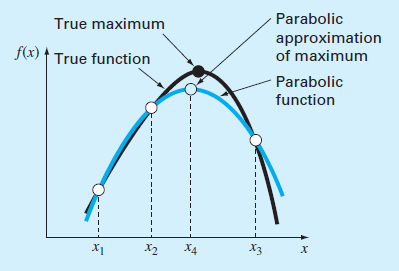
\includegraphics[width=0.5\linewidth]{fig_7_8}
	\caption{\textsf{Graphical depiction of parabolic interpolation.}}
	\label{fig:fig_7_8}
\end{figure}

\subsection{Parabolic Interpolation}

\noindent Parabolic interpolation takes advantage of the fact that a second-order polynomial often
provides a good approximation to the shape of f (x) near an optimum (Fig. 7.8).

Just as there is only one straight line connecting two points, there is only one parabola
connecting three points. Thus, if we have three points that jointly bracket an optimum, we
can fit a parabola to the points. Then we can differentiate it, set the result equal to zero, and
solve for an estimate of the optimal x. It can be shown through some algebraic manipulations
that the result is
\medskip

$x_4 = x_2 - \dfrac{1}{2}\dfrac{(x_2-x_1)^2[f(x_2)-f(x_3)]-(x_2-x_3)^2[f(x_2)-f(x_1)]}{(x_2-x_1)[f(x_2)-f(x_3)]-(x_2-x_3)[f(x_2)-f(x_1)]} $ \hfill {(7.10)}
\medskip

\noindent where $x1$, $x2$, and $x3$ are the initial guesses, and $x4$ is the value of $x$ that corresponds to the
optimum value of the parabolic fit to the guesses.

\begin{example}
	Parabolic Interpolation
	\smallskip
	
	\noindent Problem Statement:
	Use parabolic interpolation to approximate the minimum of

	$ f(x) = \dfrac{x^2}{10}-2sinx $
	\medskip
	
	with initial guesses of $x_1$ = 0, $x_2$ = 1, and $x_3$ = 4.

	\noindent Solution: The function values at the three guesses can be evaluated:
	\medskip

	$x_1 = 0$ \hspace{2cm} $f(x_1)=0$

	$x_2 = 1$ \hspace{2cm} $f(x_2)=-1.5829$

	$x_3 = 4$ \hspace{2cm} $f(x_3)=3.1136$
	\medskip

	\noindent and substituted into Eq. (7.10) to give
	\medskip
    
	$x_4=1- \dfrac{1}{2}\dfrac{(1-0)^2[-1.5829-3.1136]-(1-4)^2[-1.5829-0]}{(1-0)[-1.5829-3.1136]-(1-4)[-1.5829-0]}=1.5055 $
	\medskip

	\noindent which has a function value of f(1.5055) =-1.7691.

	Next, a strategy similar to the golden-section search can be employed to determine
	which point should be discarded. Because the function value for the new point is lower
	than for the intermediate point ($x_2$) and the new x value is to the right of the intermediate
	point, the lower guess ($x_1$) is discarded. Therefore, for the next iteration:
	\medskip

	$x_1 = 1$      \hspace{2cm} $f(x_1)=-1.5829$

	$x_2 = 1.5055$ \hspace{2cm} $f(x_2)=-1.76919$

	$x_3 = 4$      \hspace{2cm} $f(x_3)=3.1136$
	\medskip

	\noindent which can be substituted into Eq. (7.10) to give
	\medskip

	$x_4=1.5055-\dfrac{1}{2}\dfrac{(1.5055-1)^2[-1.7691-3.1136]-(1.5055-4)^2[-1.7691-(-1.5829)]}{(1.5055-1)[-1.7691-3.1136]-(1.5055-4)[-1.7691-(-1.5829)]}=1.4903 $
	\medskip

	\noindent which has a function value of f(1.4903) =-1.7714. The process can be repeated, with the
	results tabulated here:

	$$
	\begin{tabular}{|c|c|c|c|c|c|c|c|c|c|}
		\hline $i$ & $x_l$ & $f(x_l)$ & $x_2$ & $f(x_2)$ & $x_3$ & $f(x_3)$ & $x_4$ & $f(x_4)$\\
		\hline 1 & 0.0000  &  0.0000  & 1.0000 & -1.5828 & 4.0000 &  3.1136 & 1.5055 & -1.7691\\
		\hline 2 & 1.0000  & -1.5829  & 1.5055 & -1.7691 & 4.0000 &  3.1136 & 1.4903 & -1.7714\\
		\hline 3 & 1.0000  & -1.5829  & 1.4903 & -1.7714 & 1.5055 & -1.7691 & 1.4256 & -1.7757\\
		\hline 4 & 1.0000  & -1.5829  & 1.4256 & -1.7757 & 1.4903 & -1.7714 & 1.4266 & -1.7757\\
		\hline 5 & 1.4265  & -1.7757  & 1.4266 & -1.7757 & 1.4903 & -1.7714 & 1.4275 & -1.7757\\
		\hline
	\end{tabular}
	$$

	\noindent Thus, within five iterations, the result is converging rapidly on the true value of -1.7757
	at $x$ = 1.4276.
\end{example}

\subsection{MATLAB Function \texttt{fminbnd}}

\noindent Recall that in Sec. 6.4 we described Brent's method for root location, which combined several
root-finding methods into a single algorithm that balanced reliability with efficiency.
Because of these qualities, it forms the basis for the built-in MATLAB function \texttt{fzero}.

Brent also developed a similar approach for one-dimensional minimization which
forms the basis for the MATLAB \texttt{fminbnd} function. It combines the slow, dependable
golden-section search with the faster, but possibly unreliable, parabolic interpolation. It
first attempts parabolic interpolation and keeps applying it as long as acceptable results are
obtained. If not, it uses the golden-section search to get matters in hand.

A simple expression of its syntax is
\smallskip

\texttt{[xmin, fval] = fminbnd(function,x1,x2)}
\smallskip

\noindent where x and \texttt{fval} are the location and value of the minimum, \texttt{function} is the name of the
function being evaluated, and \texttt{x1} and \texttt{x2} are the bounds of the interval being searched.
\newpage

Here is a simple MATLAB session that uses \texttt{fminbnd} to solve the problem from Example 7.1.

\begin{lstlisting}[numbers=none,frame=none]
	>> g=9.81;v0=55;m=80;c=15;z0=100;
	>> z=@(t) -(z0+m/c*(v0+m*g/c)*(1-exp(-c/m*t))-m*g/c*t);
	>> [x,f]=fminbnd(z,0,8)

	x =
		3.8317
	f =
		-192.8609
\end{lstlisting}

As with \texttt{fzero}, optional parameters can be specified using \texttt{optimset}. For example,
we can display calculation details:

\begin{lstlisting}[numbers=none,frame=none]
	>> options = optimset('display','iter');
	>> fminbnd(z,0,8,options)
	Func-count 		x 			f(x) 	Procedure
		1 		3.05573 	-189.759 	initial
		2 		4.94427 	-187.19 	golden
		3 		1.88854 	-171.871 	golden
		4 		3.87544 	-192.851 	parabolic
		5 		3.85836 	-192.857 	parabolic
		6 		3.83332		-192.861 	parabolic
		7 		3.83162 	-192.861 	parabolic
		8 		3.83166 	-192.861 	parabolic
		9 		3.83169 	-192.861 	parabolic
	Optimization terminated:
	the current x satisfies the termination criteria using
	OPTIONS.TolX of 1.000000e-004
	ans =
		3.8317
\end{lstlisting}

Thus, after three iterations, the method switches from golden to parabolic, and after eight
iterations, the minimum is determined to a tolerance of 0.0001.\\

\section{MULTIDIMENSIONAL OPTIMIZATION}
\label{sec:sec_7_3}

\noindent Aside from one-dimensional functions, optimization also deals with multidimensional
functions. Recall from Fig. 7.3a that our visual image of a one-dimensional search was like
a roller coaster. For two-dimensional cases, the image becomes that of mountains and
valleys (Fig. 7.3b). As in the following example, MATLAB's graphic capabilities provide
a handy means to visualize such functions.

\begin{example}
	Visualizing a Two-Dimensional Function
	\smallskip
	
	\noindent Problem Statement:
	Use MATLAB's graphical capabilities to display the following
	function and visually estimate its minimum in the range $-2 \le x_1 \le 0$ and $0 \le x_2 \le 3$:

	$ f(x_1,x_2) = 2 + x_1 - x_2 + 2_1^2 + 2x_1x_2 + x_2^2$
	\medskip
	
	with initial guesses of $x_1$ = 0, $x_2$ = 1, and $x_3$ = 4.

	\noindent Solution: The following script generates contour and mesh plots of the function:
	\medskip

	\begin{lstlisting}[numbers=none,frame=none]
		x=linspace(-2,0,40);y=linspace(0,3,40);
		[X,Y] = meshgrid(x,y);
		Z=2+X-Y+2*X.^2+2*X.*Y+Y.^2;
		subplot(1,2,1);
		cs=contour(X,Y,Z);clabel(cs);
		xlabel('x_1');ylabel('x_2');
		title('(a) Contour plot');grid;
		subplot(1,2,2);
		cs=surfc(X,Y,Z);
		zmin=floor(min(Z));
		zmax=ceil(max(Z));
		xlabel('x_1');ylabel('x_2');zlabel('f(x_1,x_2)');
		title('(b) Mesh plot');
	\end{lstlisting}

	\noindent As displayed in Fig. 7.9, both plots indicate that function has a minimum value of about
	$f(x1, x2)$ = 0 to 1 located at about $x_1$ =-1 and $x_2$ = 1.5.

	\begin{figure}[H]
		\centering
		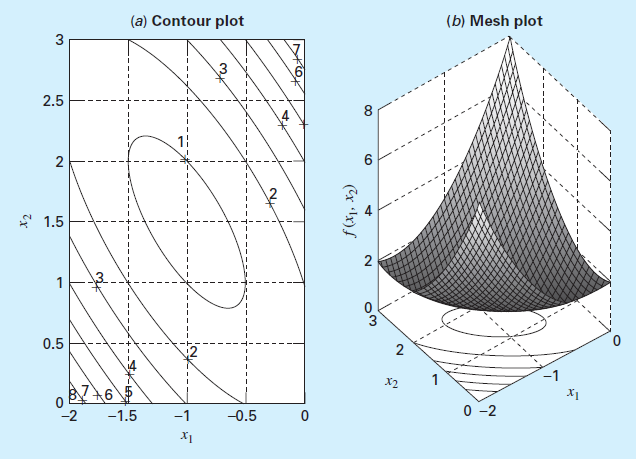
\includegraphics[width=0.75\linewidth]{fig_7_9}
		\caption{\textsf{(a) Contour and (b) mesh plots of a two-dimensional function.}}
		\label{fig:fig_7_9}
	\end{figure}
\end{example}

Techniques for multidimensional unconstrained optimization can be classified in a
number of ways. For purposes of the present discussion, we will divide them depending
on whether they require derivative evaluation. Those that require derivatives are called
\texttt{gradient}, or \texttt{descent} (or ascent), methods. The approaches that do not require derivative evaluation
are called nongradient, or direct, methods. As described next, the built-in MATLAB
function \texttt{fminsearch} is a direct method.

\subsection{MATLAB Function: \texttt{fminsearch}}

\noindent Standard MATLAB has a function \texttt{fminsearch} that can be used to determine the minimum
of a multidimensional function. It is based on the Nelder-Mead method, which is a
direct-search method that uses only function values (does not require derivatives) and
handles non-smooth objective functions. A simple expression of its syntax is
\smallskip

\texttt{\texttt{fminsearch}}
\smallskip

\noindent where \texttt{xmin} and \texttt{fval} are the location and value of the minimum, \texttt{function} is the name of
the function being evaluated, and \texttt{x0} is the initial guess. Note that \texttt{x0} can be a scalar, vector,
or a matrix.

Here is a simple MATLAB session that uses \texttt{fminsearch} to determine minimum for
the function we just graphed in Example 7.4:

\begin{lstlisting}[numbers=none,frame=none]
	>> f=@(x) 2+x(1)-x(2)+2*x(1)^2+2*x(1)*x(2)+x(2)^2;
	>> [x,fval]=fminsearch(f,[-0.5,0.5])
	x =
		-1.0000 1.5000
	fval =
		0.7500
\end{lstlisting}

\section{\textbf{CASE STUDY} - EQUILIBRIUM AND MINIMUM POTENTIAL ENERGY}
\label{sec:sec_7_4}

\textbf{Background.} As in Fig. 7.10a, an unloaded spring can be attached to a wall mount.
When a horizontal force is applied, the spring stretches. The displacement is related to the
force by $Hookes law$, $F = kx$. The potential $energy$ of the deformed state consists of the difference
between the strain energy of the spring and the work done by the force:\medskip

$PE(x) = 0.5kx^2-Fx$ \hfill{7.11}
\medskip

\begin{figure}[H]
	\centering
	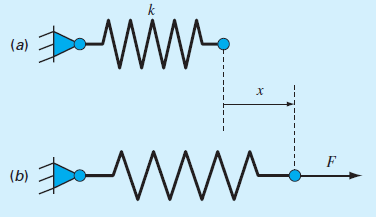
\includegraphics[width=0.5\linewidth]{fig_7_10}
	\caption{\textsf{(a) An unloaded spring attached to a wall mount. (b) Application of a horizontal force stretches
	the spring where the relationship between force and displacement is described by Hooke's law.}}
	\label{fig:fig_7_10}
\end{figure}

Equation (7.11) defines a parabola. Since the potential energy will be at a minimum at
equilibrium, the solution for displacement can be viewed as a one-dimensional optimization
problem. Because this equation is so easy to differentiate, we can solve for the displacement
as $x = F/k$. For example, if $k = 2 N/cm$ and $F = 5 N, x = 5N/(2 N/cm) = 2.5 cm.$

A more interesting two-dimensional case is shown in Fig. 7.11. In this system, there
are two degrees of freedom in that the system can move both horizontally and vertically.
In the same way that we approached the one-dimensional system, the equilibrium deformations
are the values of $x_1$ and $x_2$ that minimize the potential energy: \medskip

$PE(x_1,x_2)=0.5k_a(\sqrt{x_1^2 + (L_a-x_2)^2}-L_a)^2 + 0.5k_b(\sqrt{x_1^2+(L_b+x_2)^2}-L_b)^2-F_1x_1-F_2x_2$ \hfill{7.12}
\smallskip

\noindent If the parameters are $k_a$ = 9 N/cm, $k_b$ = 2 N/cm, $L_a$ = 10 cm, $L_b$= 10 cm, $F_1$= 2 N, and
$F_2$ = 4 N, use MATLAB to solve for the displacements and the potential energy.

\begin{figure}[H]
	\centering
	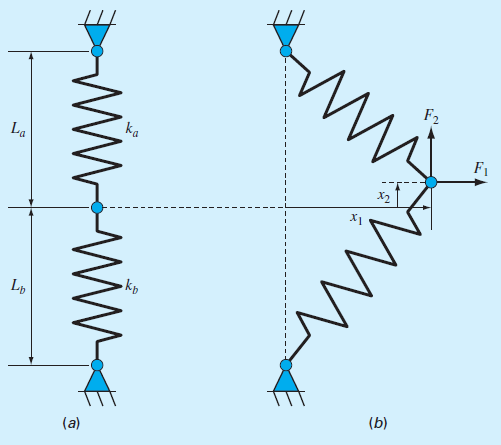
\includegraphics[width=0.5\linewidth]{fig_7_11}
	\caption{\textsf{A two-spring system: (a) unloaded and (b) loaded.}}
	\label{fig:fig_7_11}
\end{figure}

\noindent\textbf{Solution.} An M-file can be developed to hold the potential energy function:

\begin{lstlisting}[numbers=none,frame=none]
	function p=PE(x,ka,kb,La,Lb,F1,F2)
	PEa=0.5*ka*(sqrt(x(1)^2+(La-x(2))^2)-La)^2;
	PEb=0.5*kb*(sqrt(x(1)^2+(Lb+x(2))^2)-Lb)^2;
	W=F1*x(1)+F2*x(2);
	p=PEa+PEb-W;
\end{lstlisting}

\noindent The solution can be obtained with the \texttt{fminsearch} function:

\begin{lstlisting}[numbers=none,frame=none]
	>> ka=9;kb=2;La=10;Lb=10;F1=2;F2=4;
	>> [x,f]=fminsearch(@PE,[-0.5,0.5],[],ka,kb,La,Lb,F1,F2)
	x =
		4.9523 	1.2769
	f =
		-9.6422
\end{lstlisting}

Thus, at equilibrium, the potential energy is -9.6422 N· cm. The connecting point is
located 4.9523 cm to the right and 1.2759 cm above its original position.\bigskip
\newpage

\noindent\textbf{PROBLEMS}

\begin{multicols}{2}
	\noindent\textbf{7.1} Perform three iterations of the Newton-Raphson method
	to determine the root of Eq. (E7.1.1). Use the parameter values
	from Example 7.1 along with an initial guess of $t$ = 3 s.

	\noindent\textbf{7.2} Given the formula

	\noindent $f(x) = -x^2 + 8x - 12$

	\noindent(a) Determine the maximum and the corresponding value of
	$x$ for this function analytically (i.e., using differentiation).
	(b) Verify that Eq. (7.10) yields the same results based on
	initial guesses of $x_1$ = 0, $x_2$ = 2, and $x_3$ = 6.

	\noindent\textbf{7.3} Consider the following function:

	\noindent$f(x) = 3 + 6x + 5x^2 + 3x^3 + 4x^4$

	\noindent Locate the minimum by finding the root of the derivative of
	this function. Use bisection with initial guesses of $x_l= -2$ and $x_u = 1$.

	\noindent\textbf{7.4} Given

	\noindent$f(x) = -1.5x^6 - 2x^4 + 12x$

	\noindent  (a) Plot the function.

	\noindent(b) Use analytical methods to prove that the function is concave
	for all values of $x$.

	\noindent(c) Differentiate the function and then use a root-location
	method to solve for the maximum $f(x)$ and the corresponding value of $x$.

	\noindent\textbf{7.5} Solve for the value of x that maximizes $f(x)$ in Prob. 7.4
	using the golden-section search. Employ initial guesses of $x_l$ = 0 and $x_u$ = 2, 
	and perform three iterations.

	\noindent\textbf{7.6} Repeat Prob. 7.5, except use parabolic interpolation.
	Employ initial guesses of $x_1$ = 0, $x_2$ = 1, and $x_3$ = 2, and perform three iterations.

	\noindent\textbf{7.7} Employ the following methods to find the maximum of

	\noindent $f (x) = 4x - 1.8x^2 + 1.2x^3 - 0.3x^4$

	\noindent(a)Golden-section search ($x_l$ = - 2, $x_u$ = 4, $\epsilon_s$ = 1\%). 

	\noindent(b)Parabolic interpolation ($x_1$ = 1.75, $x_2$ = 2, $x_3$ = 2.5, iterations = 5).

	\noindent\textbf{7.8} Consider the following function:

	\noindent $f(x) = x^4 + 2x^3 + 8x^2 + 5x$

	\noindent Use analytical and graphical methods to show the function
	has a minimum for some value of $x$ in the range

	$-2 \le x \le 1.$

	\noindent\textbf{7.9} Employ the following methods to find the minimum of
	the function from Prob. 7.8:

	\noindent (a) Golden-section search ($x_l$ = -2, $x_u$= 1, $\epsilon_s$ = 1\%).

	\noindent (b) Parabolic interpolation ($x_1$= -2, $x_2$= -1, $x_3$= 1, iterations = 5).

	\noindent\textbf{7.10} Consider the following function:

	\noindent$f(x)=2x+\dfrac{3}{x}$

	\noindent Perform 10 iterations of parabolic interpolation to locate
	the minimum. Comment on the convergence of your results
	($x_1$ = 0.1, $x_2$ = 0.5, $x_3$ = 5)

	\noindent\textbf{7.11} Develop a single script to (a) generate contour and
	mesh subplots of the following temperature field in a similar
	fashion to Example 7.4:

	\noindent $T(x, y) = 2x^2 + 3y^2 - 4xy - y - 3x$

	\noindent and (b) determine the minimum with \texttt{fminsearch}.

	\noindent\textbf{7.12} The head of a groundwater aquifer is described in
	Cartesian coordinates by

	\noindent $h(x,y) = \dfrac{1}{1+x^2 + y^2 + x +xy}$

	\noindent Develop a single script to (a) generate contour and mesh
	subplots of the function in a similar fashion to Example 7.4,
	and (b) determine the maximum with fminsearch.

	\noindent\textbf{7.13} Recent interest in competitive and recreational cycling
	has meant that engineers have directed their skills toward the
	design and testing of mountain bikes (Fig. P7.13a). Suppose
	that you are given the task of predicting the horizontal
	and vertical displacement of a bike bracketing system in
	response to a force. Assume the forces you must analyze can
	be simplified as depicted in Fig. P7.13b. You are interested

	\begin{center}
	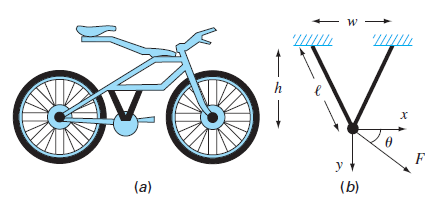
\includegraphics[width=1\linewidth]{fig_P7_13}
	\textsf{(a) A mountain bike along with (b) a free-body diagram
	for a part of the frame.}
	\end{center}

	\noindent in testing the response of the truss to a force exerted in any
	number of directions designated by the angle $\theta$. The
	parameters for the problem are $E$ = Young's modulus
	= $2 \times 10^11$ Pa, A = cross-sectional area = 0.0001 $m^2$, $w$ =
	width = 0.44 m, $l$ = length = 0.56 m, and $h$ = height
	= 0.5 m. The displacements $x$ and $y$ can be solved by determining
	the values that yield a minimum potential energy.
	Determine the displacements for a force of 10,000 N and a
	range of $\theta$'s from 0° (horizontal) to 90° (vertical).

	\noindent \textbf{7.14} As electric current moves through a wire (Fig. P7.14), heat generated by resistance is conducted through a layer of insulation and then convected to the surrounding air. The steady-state temperature of the wire can be computed as
	$$
	T=T_{\mathrm{air}}+\frac{q}{2 \pi}\left[\frac{1}{k} \ln \left(\frac{r_{w}+r_{i}}{r_{w}}\right)+\frac{1}{h} \frac{1}{r_{w}+r_{i}}\right]
	$$
	Determine the thickness of insulation $r_{i}(\mathrm{~m})$ that minimizes the wire's temperature given the following parameters: $q=$ heat generation rate $=75 \mathrm{~W} / \mathrm{m}, r_{w}=$ wire radius $=6 \mathrm{~mm}$, $k=$ thermal conductivity of insulation $=0.17 \mathrm{~W} /(\mathrm{m} \mathrm{K})$,
	$h=$ convective heat transfer coefficient $=12 \mathrm{~W} /\left(\mathrm{m}^{2} \mathrm{~K}\right)$, and $T_{\text {air }}=$ air temperature $=293 \mathrm{~K}$.
	
	\begin{center}
	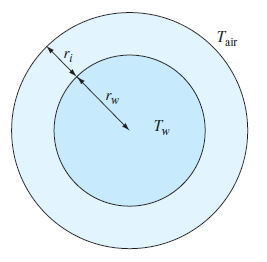
\includegraphics[width=0.65\linewidth]{fig_P7_14}

	\textsf{Cross-section of an insulated wire.}
	\end{center}

	\newpage
	\noindent \textbf{7.15} Develop an M-file that is expressly designed to locate a maximum with the golden-section search. In other words, set if up so that it directly finds the maximum rather than finding the minimum of $-f(x)$. The function should have the following features:

	- Iterate until the relative error falls below a stopping criterion or exceeds a maximum number of iterations.

	- Return both the optimal $x$ and $f(x)$.

	\noindent Test your program with the same problem as Example 7.1.
	
	\noindent \textbf{7.16} Develop an M-file to locate a minimum with the golden-section search. Rather than using the maximum iterations and Eq. (7.9) as the stopping criteria, determine the number of iterations needed to attain a desired tolerance. Test your function by solving Example $7.2$ using $E_{a, d}=0.0001$. 
	
	\noindent \textbf{7.17} Develop an M-file to implement parabolic interpolation to locate a minimum. The function should have the following features:
	\begin{itemize}
		\item Base it on two initial guesses, and have the program generate the third initial value at the midpoint of the interval.
		\item Check whether the guesses bracket a maximum. If not, the function should not implement the algorithm, but should return an error message.
		\item Iterate until the relative error falls below a stopping criterion or exceeds a maximum number of iterations.	
		\item Return both the optimal $x$ and $f(x)$.
	\end{itemize}
	
	\noindent Test your program with the same problem as Example 7.3.
	
	\noindent \textbf{7.18} Pressure measurements are taken at certain points behind an airfoil over time. These data best fit the curve $y=6 \cos x-1.5 \sin x$ from $x=0$ to $6 \mathrm{~s}$. Use four iterations of the golden-search method to find the minimum pressure. Set $x_{l}=2$ and $x_{u}=4$
	
	\noindent \textbf{7.19} The trajectory of a ball can be computed with
	$$
	y=\left(\tan \theta_{0}\right) x-\frac{g}{2 v_{0}^{2} \cos ^{2} \theta_{0}} x^{2}+y_{0}
	$$
	where $y=$ the height $(\mathrm{m}), \theta_{0}=$ the initial angle (radians), $v_{0}=$ the initial velocity $(\mathrm{m} / \mathrm{s}), g=$ the gravitational constant $=9.81 \mathrm{~m} / \mathrm{s}^{2}$, and $y_{0}=$ the initial height ( $\left.\mathrm{m}\right)$. Use the golden-section search to determine the maximum height given $y_{0}=1 \mathrm{~m}, v_{0}=25 \mathrm{~m} / \mathrm{s}$, and $\theta_{0}=50^{\circ}$. Iterate until the approximate error falls below $\varepsilon_{s}=1 \%$ using initial guesses of $x_{l}=0$ and $x_{u}=60 \mathrm{~m}$.
	
	\noindent \textbf{7.20} The deflection of a uniform beam subject to a linearly increasing distributed load can be computed as
	$$
	y=\frac{w_{0}}{120 E I L}\left(-x^{5}+2 L^{2} x^{3}-L^{4} x\right)
	$$
	Given that $L=600 \mathrm{~cm}, E=50,000 \mathrm{kN} / \mathrm{cm}^{2}, I=30,000 \mathrm{~cm}^{4}$, and $w_{0}=2.5 \mathrm{kN} / \mathrm{cm}$, determine the point of maximum deflection (a) graphically, (b) using the golden-section search until the approximate error falls below $\varepsilon_{s}=1 \%$ with initial guesses of $x_{1}=0$ and $x_{u}=L$.
	
	\noindent \textbf{7.21} A object with a mass of $90 \mathrm{~kg}$ is projected upward from the surface of the earth at a velocity of $60 \mathrm{~m} / \mathrm{s}$. If the object is subject to linear drag $(c=15 \mathrm{~kg} / \mathrm{s})$, use the goldensection search to determine the maximum height the object attains.

	\noindent \textbf{7.22} The normal distribution is a bell-shaped curve defined by
	$$
	y=e^{-x^{2}}
	$$
	Use the golden-section search to determine the location of the inflection point of this curve for positive $x$.
	\noindent \textbf{7.23} Use the fminsearch function to determine the minimum of
	$$
	f(x, y)=2 y^{2}-2.25 x y-1.75 y+1.5 x^{2}
	$$
	\noindent \textbf{7.24} Use the fminsearch function to determine the maximum of
	$$
	f(x, y)=4 x+2 y+x^{2}-2 x^{4}+2 x y-3 y^{2}
	$$
	\noindent \textbf{7.25} Given the following function:
	$$
	f(x, y)=-8 x+x^{2}+12 y+4 y^{2}-2 x y
	$$
	Determine the minimum (a) graphically, (b) numerically with the fminsearch function, and (c) substitute the result of (b) back into the function to determine the minimum $f(x, y)$.
	
	\noindent \textbf{7.26} The specific growth rate of a yeast that produces an antibiotic is a function of the food concentration $c$ :
	$$
	g=\frac{2 c}{4+0.8 c+c^{2}+0.2 c^{3}}
	$$
	As depicted in Fig. P7.26, growth goes to zero at very low concentrations due to food limitation. It also goes to zero at high concentrations due to toxicity effects. Find the value of $c$ at which growth is a maximum.
	
	\begin{center}
	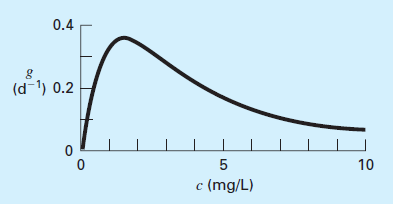
\includegraphics[width=1\linewidth]{fig_P7_26}
	\textsf{The specific growth rate of a yeast that produces an
	antibiotic versus the food concentration.}
	\end{center}

	\noindent \textbf{7.27} A compound A will be converted into B in a stirred tank reactor. The product B and unreacted A are purified in a separation unit. Unreacted $\mathrm{A}$ is recycled to the reactor. A process engineer has found that the initial cost of the system is a function of the conversion $x_{A}$. Find the conversion that will result in the lowest cost system. $C$ is a proportionality constant.
	$$
	\text { Cost }=C\left[\left(\frac{1}{\left(1-x_{A}\right)^{2}}\right)^{0.6}+6\left(\frac{1}{x_{A}}\right)^{0.6}\right]
	$$
	\newpage

	\noindent \textbf{7.28} A finite-element model of a cantilever beam subject to loading and moments (Fig. P7.28) is given by optimizing
	$$
	f(x, y)=5 x^{2}-5 x y+2.5 y^{2}-x-1.5 y
	$$
	where $x=$ end displacement and $y=$ end moment. Find the values of $x$ and $y$ that minimize $f(x, y)$.
	
	\begin{center}
	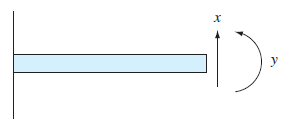
\includegraphics[width=0.7\linewidth]{fig_P7_28}

	\textsf{A cantilever beam.}
	\end{center}

	\noindent \textbf{7.29} The Streeter-Phelps model can be used to compute the dissolved oxygen concentration in a river below a point discharge of sewage (Fig. P7.29),
	$$
	\begin{aligned}
	o=& o_{s}-\frac{k_{d} L_{o}}{k_{d}+k_{s}-k_{a}}\left(e^{-k_{a} t}-e^{-\left(k_{d}+k_{s}\right) t}\right) \\
	&-\frac{S_{b}}{k_{a}}\left(1-e^{-k_{a} t}\right)
	\end{aligned}
	$$
	where $o=$ dissolved oxygen concentration $(\mathrm{mg} / \mathrm{L}), o_{s}=$ oxygen saturation concentration $(\mathrm{mg} / \mathrm{L}), t=$ travel time $(\mathrm{d})$, $L_{o}=$ biochemical oxygen demand (BOD) concentration at the mixing point $(\mathrm{mg} / \mathrm{L}), k_{d}=$ rate of decomposition of BOD $\left(\mathrm{d}^{-1}\right), k_{s}=$ rate of settling of BOD $\left(\mathrm{d}^{-1}\right), k_{a}=$ reaeration rate $\left(\mathrm{d}^{-1}\right)$, and $S_{b}=$ sediment oxygen demand $(\mathrm{mg} / \mathrm{L} / \mathrm{d})$.
	As indicated in Fig. P7.29, Eq. (P7.29) produces an oxygen "sag" that reaches a critical minimum level $o_{c}$, some travel time $t_{c}$ below the point discharge. This point is called "critical" because it represents the location where biota that depend on oxygen (like fish) would be the most stressed. Determine the critical travel time and concentration, given the following values:
	$$
	\begin{array}{lll}
	o_{s}=10 \mathrm{mg} / \mathrm{L} & k_{d}=0.1 \mathrm{~d}^{-1} & k_{a}=0.6 \mathrm{~d}^{-1} \\
	k_{s}=0.05 \mathrm{~d}^{-1} & L_{o}=50 \mathrm{mg} / \mathrm{L} & S_{b}=1 \mathrm{mg} / \mathrm{L} / \mathrm{d}
	\end{array}
	$$

	\begin{center}
	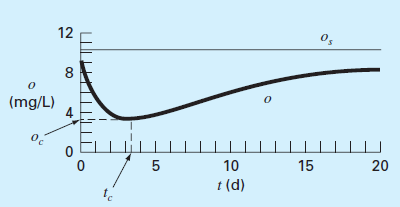
\includegraphics[width=0.7\linewidth]{fig_P7_29}
	
	\textsf{A dissolved oxygen “sag” below a point discharge of
	sewage into a river.}
	\end{center}

	\noindent \textbf{7.30} The two-dimensional distribution of pollutant concentration in a channel can be described by
	$c(x, y)=7.9+0.13 x+0.21 y-0.05 x^{2}$ $-0.016 y^{2}-0.007 x y$ the function and the knowledge that the peak lies within the bounds $-10 \leq x \leq 10$ and $0 \leq y \leq 20$.
	
	\noindent \textbf{7.31} A total charge $Q$ is uniformly distributed around a ringshaped conductor with radius $a$. A charge $q$ is located at a distance $x$ from the center of the ring (Fig. P7.31). The force exerted on the charge by the ring is given by
	$$
	F=\frac{1}{4 \pi e_{0}} \frac{q Q x}{\left(x^{2}+a^{2}\right)^{3 / 2}}
	$$
	where $e_{0}=8.85 \times 10^{-12} \mathrm{C}^{2} /\left(\mathrm{N} \mathrm{m}{ }^{2}\right), q=Q=2 \times 10^{-5} \mathrm{C}$, and $a=0.9 \mathrm{~m}$. Determine the distance $x$ where the force is a maximum.
	
	\begin{center}
	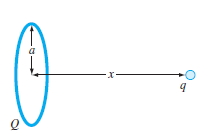
\includegraphics[width=0.7\linewidth]{fig_P7_31}
	\end{center}

	\noindent \textbf{7.32} The torque transmitted to an induction motor is a function of the slip between the rotation of the stator field and the rotor speed $s$, where slip is defined as
	$$
	s=\frac{n-n_{R}}{n}
	$$
	where $n=$ revolutions per second of rotating stator speed and $n_{R}=$ rotor speed. Kirchhoff's laws can be used to show that the torque (expressed in dimensionless form) and slip are related by
	$$
	T=\frac{15 s(1-s)}{(1-s)\left(4 s^{2}-3 s+4\right)}
	$$
	Figure P7.32 shows this function. Use a numerical method to determine the slip at which the maximum torque occurs. 
	
	\begin{center}
	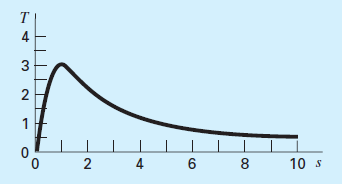
\includegraphics[width=0.7\linewidth]{fig_P7_32}
		
	\textsf{Torque transmitted to an inductor as a function of slip.}
	\end{center}

	\noindent \textbf{7.33} The total drag on an airfoil can be estimated by
	$$
	D=0.01 \sigma V^{2}+\frac{0.95}{\sigma}\left(\frac{W}{V}\right)^{2}
	$$
	Friction Lift
	where $D=$ drag, $\sigma=$ ratio of air density between the flight altitude and sea level, $W=$ weight, and $V=$ velocity. As seen in Fig. P7.33, the two factors contributing to drag are affected differently as velocity increases. Whereas friction drag increases with velocity, the drag due to lift decreases. The combination of the two factors leads to a minimum drag.
	
	(a) If $\sigma=0.6$ and $W=16,000$, determine the minimum drag and the velocity at which it occurs.
	
	(b) In addition, develop a sensitivity analysis to determine how this optimum varies in response to a range of $W=12,000$ to 20,000 with $\sigma=0.6$.
	
	\begin{center}
	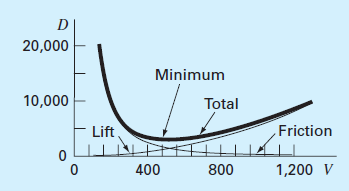
\includegraphics[width=0.7\linewidth]{fig_P7_33}
			
	\textsf{Plot of drag versus velocity for an airfoil.}
	\end{center}

	\noindent \textbf{7.34} Roller bearings are subject to fatigue failure caused by large contact loads $F$ (Fig. P7.34). The problem of finding the location of the maximum stress along the $x$ axis can be shown to be equivalent to maximizing the function:
	$$
	f(x)=\frac{0.4}{\sqrt{1+x^{2}}}-\sqrt{1+x^{2}}\left(1-\frac{0.4}{1+x^{2}}\right)+x
	$$
	Find the $x$ that maximizes $f(x)$.

	\begin{center}
	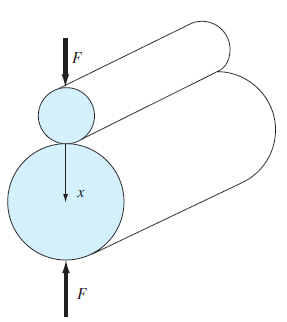
\includegraphics[width=0.7\linewidth]{fig_P7_34}
				
	\textsf{Plot of drag versus velocity for an airfoil.}
	\end{center}

	\noindent \textbf{7.35} In a similar fashion to the case study described in Sec. 7.4, develop the potential energy function for the system depicted in Fig. P7.35. Develop contour and surface
	plots in MATLAB. Minimize the potential energy function to determine the equilibrium displacements $x_{1}$ and $x_{2}$ given the forcing function $F=100 \mathrm{~N}$ and the parameters $k_{a}=20$ and $k_{b}=15 \mathrm{~N} / \mathrm{m}$.
	
	\begin{center}
	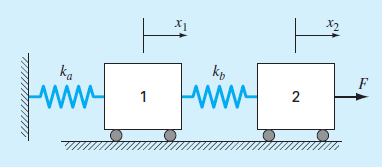
\includegraphics[width=0.7\linewidth]{fig_P7_35}
				
	\textsf{Two frictionless masses connected to a wall by a pair of
	linear elastic springs.}
	\end{center}

	\noindent \textbf{7.36} As an agricultural engineer, you must design a trapezoidal open channel to carry irrigation water (Fig. P7.36). Determine the optimal dimensions to minimize the wetted perimeter for a cross-sectional area of $50 \mathrm{~m}^{2}$. Are the relative dimensions universal?
	
	\begin{center}
	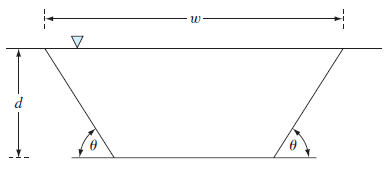
\includegraphics[width=0.7\linewidth]{fig_P7_36}
	\end{center}

	\noindent \textbf{7.37} Use the function \texttt{fminsearch} to determine the length of the shortest ladder that reaches from the ground over the fence to the building's wall (Fig. P7.37). Test it for the case where $h=d=4 \mathrm{~m}$.

	\begin{center}
	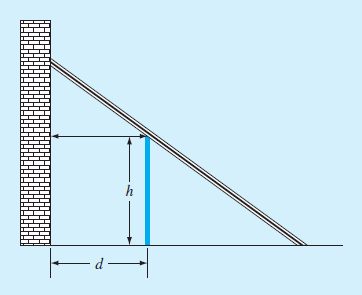
\includegraphics[width=0.7\linewidth]{fig_P7_37}
					
	\textsf{A ladder leaning against a fence and just touching a wall.}
	\end{center}

	\noindent \textbf{7.38} The length of the longest ladder that can negotiate the corner depicted in Fig. P7.38 can be determined by computing the value of $\theta$ that minimizes the following function:
	$$
	L(\theta)=\frac{w_{1}}{\sin \theta}+\frac{w_{2}}{\sin (\pi-\alpha-\theta)}
	$$
	For the case where $w_{1}=w_{2}=2 \mathrm{~m}$, use a numerical method described in this chapter (including MATLAB's built-in capabilities) to develop a plot of $L$ versus a range of $\alpha$ 's from 45 to $135^{\circ}$.

	\begin{center}
	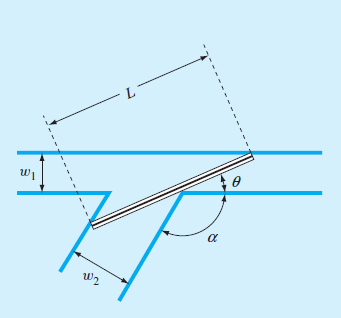
\includegraphics[width=0.7\linewidth]{fig_P7_38}
						
	\textsf{A ladder negotiating a corner formed by two hallways.}
	\end{center}




\end{multicols}

\end{document}